%!TEX root = ../OGUSAdoc.tex

We start the \ogindia section on modeling the household with a description of the demographics of the model. \citet{Nishiyama:2015} and \citet{DeBackerEtAl:2017} have recently shown that demographic dynamics are likely the biggest influence on macroeconomic time series, exhibiting more influence than fiscal variables or household preference parameters.

In this chapter, we characterize the equations and parameters that govern the transition dynamics of the population distribution by age. In \ogindia, we take the approach of taking mortality rates and fertility rates from outside estimates. But we estimate our immigration rates as residuals using the mortality rates, fertility rates, and at least two consecutive periods of population distribution data. This approach makes sense if one modeling a country in which in one is not confident in the immigration rate data. If the country has good immigration data, then the immigration residual approach we describe below can be skipped.

We define $\omega_{s,t}$ as the number of households of age $s$ alive at time $t$. A measure $\omega_{1,t}$ of households is born in each period $t$ and live for up to $E+S$ periods, with $S\geq 4$.\footnote{Theoretically, the model works without loss of generality for $S\geq 3$. However, because we are calibrating the ages outside of the economy to be one-fourth of $S$ (e.g., ages 21 to 100 in the economy, and ages 1 to 20 outside of the economy), it is convenient for $S$ to be at least 4.} Households are termed ``youth'', and do not participate in market activity during ages $1\leq s\leq E$. The households enter the workforce and economy in period $E+1$ and remain in the workforce until they unexpectedly die or live until age $s=E+S$. We model the population with households age $s\leq E$ outside of the workforce and economy in order most closely match the empirical population dynamics.

The population of agents of each age in each period $\omega_{s,t}$ evolves according to the following function,
\begin{equation}\label{EqPopLawofmotion}
  \begin{split}
    \omega_{1,t+1} &= (1 - \rho_0)\sum_{s=1}^{E+S} f_s\omega_{s,t} + i_1\omega_{1,t}\quad\forall t \\
    \omega_{s+1,t+1} &= (1 - \rho_s)\omega_{s,t} + i_{s+1}\omega_{s+1,t}\quad\forall t\quad\text{and}\quad 1\leq s \leq E+S-1
  \end{split}
\end{equation}
where $f_s\geq 0$ is an age-specific fertility rate, $i_s$ is an age-specific net immigration rate, $\rho_s$ is an age-specific mortality hazard rate, and $\rho_0$ is an infant mortality rate.\footnote{The parameter $\rho_s$ is the probability that a household of age $s$ dies before age $s+1$.} The total population in the economy $N_t$ at any period is simply the sum of households in the economy, the population growth rate in any period $t$ from the previous period $t-1$ is $g_{n,t}$, $\tilde{N}_t$ is the working age population, and $\tilde{g}_{n,t}$ is the working age population growth rate in any period $t$ from the previous period $t-1$.
\begin{equation}\label{EqPopN}
  N_t\equiv\sum_{s=1}^{E+S} \omega_{s,t} \quad\forall t
\end{equation}
\begin{equation}\label{EqPopGrowth}
  g_{n,t+1} \equiv \frac{N_{t+1}}{N_t} - 1 \quad\forall t
\end{equation}
\begin{equation}\label{EqPopNtil}
  \tilde{N}_t\equiv\sum_{s=E+1}^{E+S} \omega_{s,t} \quad\forall t
\end{equation}
\begin{equation}\label{EqPopGrowthTil}
  \tilde{g}_{n,t+1} \equiv \frac{\tilde{N}_{t+1}}{\tilde{N}_t} - 1 \quad\forall t
\end{equation}
We discuss the approach to estimating fertility rates $f_s$, mortality rates $\rho_s$, and immigration rates $i_s$ in Sections \ref{SecDemogFert}, \ref{SecDemogMort}, and \ref{SecDemogImm}.


\section{Fertility rates}\label{SecDemogFert}

  In \ogindia, we assume that the fertility rates for each age cohort $f_s$ are constant across time. However, this assumption is conceptually straightforward to relax. Our data for U.S. fertility rates by age come from \citet[Table 3, p. 18]{MartinEtAl:2015} National Vital Statistics Report, which is final fertility rate data for 2013. Figure \ref{FigFertRates} shows the fertility-rate data and the estimated average fertility rates for $E+S=100$.

  \begin{figure}[htbp]\centering \captionsetup{width=4.0in}
    \caption{\label{FigFertRates}\textbf{Fertility rates by age ($f_s$) for $E+S=100$}}
    \fbox{\resizebox{4.0in}{3.0in}{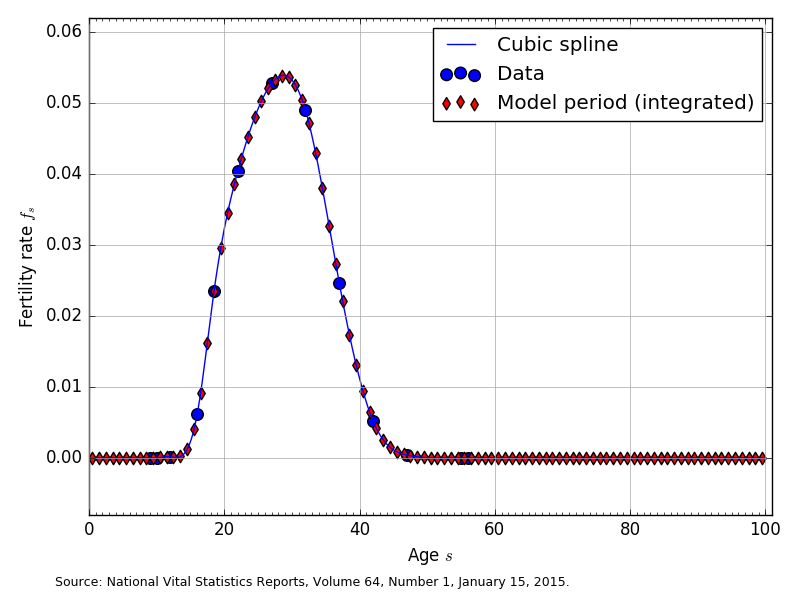
\includegraphics{./images/fert_rates.png}}}
  \end{figure}

  The large blue circles are the 2013 U.S. fertility rate data from \citet{MartinEtAl:2015}. These are 9 fertility rates $[0.3, 12.3, 47.1, 80.7, 105.5, 98.0, 49.3, 10.4, 0.8]$ that correspond to the midpoint ages of the following age (in years) bins $[10-14, 15-17, 18-19, 20-24, 25-29, 30-34, 35-39, 40-44, 45-49]$. In order to get our cubic spline interpolating function to fit better at the endpoints we added to fertility rates of zero to ages 9 and 10, and we added two fertility rates of zero to ages 55 and 56. The blue line in Figure \ref{FigFertRates} shows the cubic spline interpolated function of the data.

  The red diamonds in Figure \ref{FigFertRates} are the average fertility rate in age bins spanning households born at the beginning of period 1 (time = 0) and dying at the end of their 100th year. Let the total number of model years that a household lives be $E+S\leq 100$. Then the span from the beginning of period 1 (the beginning of year 0) to the end of period 100 (the end of year 99) is divided up into $E+S$ bins of equal length. We calculate the average fertility rate in each of the $E+S$ model-period bins as the average population-weighted fertility rate in that span. The red diamonds in Figure \ref{FigFertRates} are the average fertility rates displayed at the midpoint in each of the $E+S$ model-period bins.


\section{Mortality rates}\label{SecDemogMort}

  The mortality rates in our model $\rho_s$ are a one-period hazard rate and represent the probability of dying within one year, given that an household is alive at the beginning of period $s$. We assume that the mortality rates for each age cohort $\rho_s$ are constant across time. The infant mortality rate of $\rho_0=0.00587$ comes from the 2015 U.S. CIA World Factbook. Our data for U.S. mortality rates by age come from the Actuarial Life Tables of the U.S. Social Security Administration \citep[see][]{SocSec:2015}, from which the most recent mortality rate data is for 2011. Figure \ref{FigMortRates} shows the mortality rate data and the corresponding model-period mortality rates for $E+S=100$.

  \begin{figure}[htbp]\centering \captionsetup{width=4.0in}
    \caption{\label{FigMortRates}\textbf{Mortality rates by age ($\rho_s$) for $E+S=100$}}
    \fbox{\resizebox{4.0in}{3.0in}{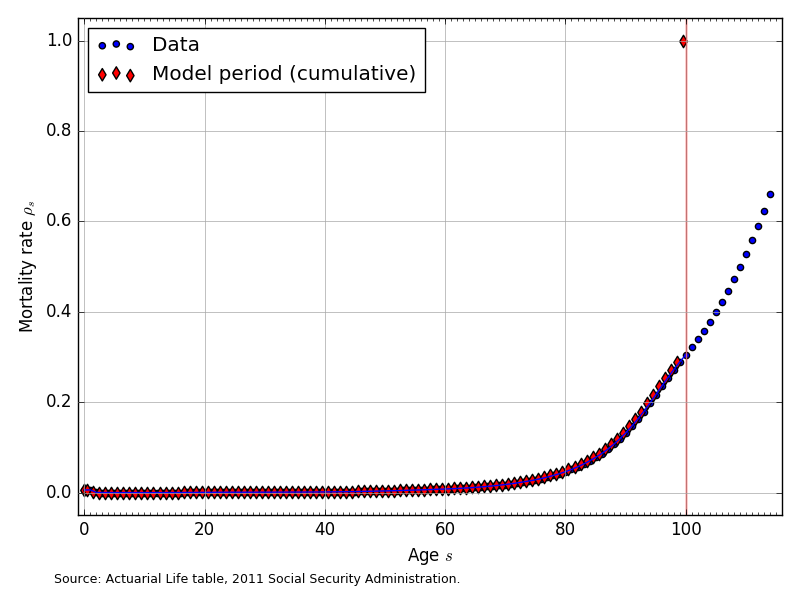
\includegraphics{./images/mort_rates.png}}}
  \end{figure}

  The mortality rates in Figure \ref{FigMortRates} are a population-weighted average of the male and female mortality rates reported in \citet{SocSec:2015}. Figure \ref{FigMortRates} also shows that the data provide mortality rates for ages up to 111-years-old. We truncate the maximum age in years in our model to 100-years old. In addition, we constrain the mortality rate to be 1.0 or 100 percent at the maximum age of 100.


\section{Immigration rates}\label{SecDemogImm}

  Because of the difficulty in getting accurate immigration rate data by age, we estimate the immigration rates by age in our model $i_s$ as the average residual that reconciles the current-period population distribution with next period's population distribution given fertility rates $f_s$ and mortality rates $\rho_s$. Solving equations \eqref{EqPopLawofmotion} for the immigration rate $i_s$ gives the following characterization of the immigration rates in given population levels in any two consecutive periods $\omega_{s,t}$ and $\omega_{s,t+1}$ and the fertility rates $f_s$ and mortality rates $\rho_s$.

  \begin{equation}\label{EqPopImmRates}
    \begin{split}
      i_1 &= \frac{\omega_{1,t+1} - (1 - \rho_0)\sum_{s=1}^{E+S}f_s\omega_{s,t}}{\omega_{1,t}}\quad\forall t \\
      i_{s+1} &= \frac{\omega_{s+1,t+1} - (1 - \rho_s)\omega_{s,t}}{\omega_{s+1,t}}\qquad\qquad\forall t\quad\text{and}\quad 1\leq s \leq E+S-1
    \end{split}
  \end{equation}

  \begin{figure}[htbp]\centering \captionsetup{width=4.0in}
    \caption{\label{FigImmRates}\textbf{Immigration rates by age ($i_s$), residual, $E+S=100$}}
    \fbox{\resizebox{4.0in}{3.0in}{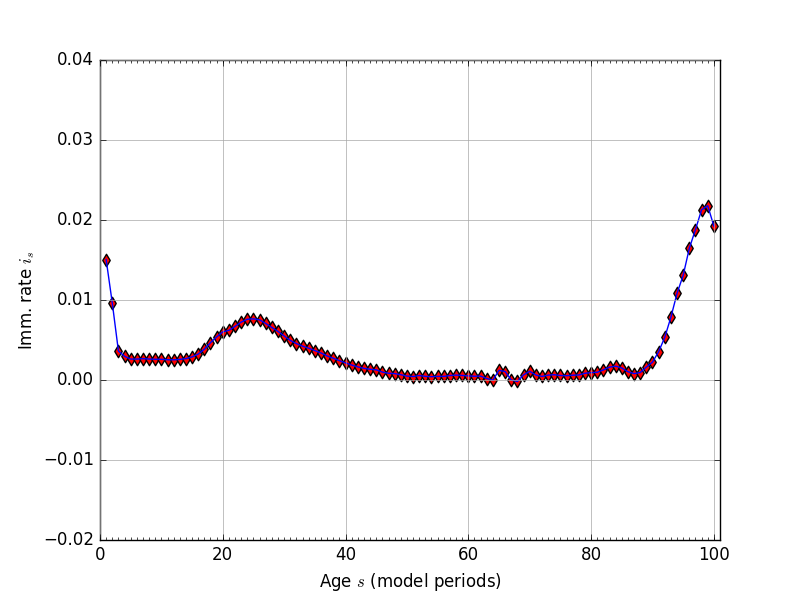
\includegraphics{./images/imm_rates_orig.png}}}
  \end{figure}

  We calculate our immigration rates for three different consecutive-year-periods of population distribution data (2010 through 2013). Our four years of population distribution by age data come from \citet{Census:2015}. The immigration rates $i_s$ that we use in our model are the the residuals described in \eqref{EqPopImmRates} averaged across the three periods. Figure \ref{FigImmRates} shows the estimated immigration rates for $E+S=100$ and given the fertility rates from Section \ref{SecDemogFert} and the mortality rates from Section \ref{SecDemogMort}.

  At the end of Section \ref{SecDemogPopSSTP}, we describe a small adjustment that we make to the immigration rates after a certain number of periods in order to make computation of the transition path equilibrium of the model compute more robustly.


\section{Population steady-state and transition path}\label{SecDemogPopSSTP}

  This model requires information about mortality rates $\rho_s$ in order to solve for the household's problem each period. It also requires the steady-state stationary population distribution $\bar{\omega}_{s}$ and population growth rate $\bar{g}_n$ as well as the full transition path of the stationary population distribution $\hat{\omega}_{s,t}$ and population grow rate $\tilde{g}_{n,t}$ from the current state to the steady-state. To solve for the steady-state and the transition path of the stationary population distribution, we write the stationary population dynamic equations \eqref{EqPopLawofmotionStat} and their matrix representation \eqref{EqPopLOMstatmat}.
  \begin{equation}\label{EqPopLawofmotionStat}
    \begin{split}
      \hat{\omega}_{1,t+1} &= \frac{(1-\rho_0)\sum_{s=1}^{E+S} f_s\hat{\omega}_{s,t} + i_1\hat{\omega}_{1,t}}{1+\tilde{g}_{n,t+1}}\quad\forall t \\
      \hat{\omega}_{s+1,t+1} &= \frac{(1 - \rho_s)\hat{\omega}_{s,t} + i_{s+1}\hat{\omega}_{s+1,t}}{1+\tilde{g}_{n,t+1}}\qquad\quad\:\forall t\quad\text{and}\quad 1\leq s \leq E+S-1
    \end{split}
  \end{equation}
  \begin{equation}\label{EqPopLOMstatmat}
    \begin{split}
      & \begin{bmatrix}
        \hat{\omega}_{1,t+1} \\ \hat{\omega}_{2,t+1} \\ \hat{\omega}_{2,t+1} \\ \vdots \\ \hat{\omega}_{E+S-1,t+1} \\ \hat{\omega}_{E+S,t+1}
      \end{bmatrix}= \frac{1}{1 + g_{n,t+1}} \times ... \\
      & \begin{bmatrix}
        (1-\rho_0)f_1+i_1 & (1-\rho_0)f_2 & (1-\rho_0)f_3 & \hdots & (1-\rho_0)f_{E+S-1} & (1-\rho_0)f_{E+S} \\
        1-\rho_1 & i_2 & 0 & \hdots & 0 & 0 \\
        0 & 1-\rho_2 & i_3 & \hdots & 0 & 0 \\
        \vdots & \vdots & \vdots & \ddots & \vdots & \vdots \\
        0 & 0 & 0 & \hdots & i_{E+S-1} & 0 \\
        0 & 0 & 0 & \hdots & 1-\rho_{E+S-1} & i_{E+S}
      \end{bmatrix}
      \begin{bmatrix}
        \hat{\omega}_{1,t} \\ \hat{\omega}_{2,t} \\ \hat{\omega}_{2,t} \\ \vdots \\ \hat{\omega}_{E+S-1,t} \\ \hat{\omega}_{E+S,t}
      \end{bmatrix}
    \end{split}
  \end{equation}
  We can write system \eqref{EqPopLOMstatmat} more simply in the following way.
  \begin{equation}\label{EqPopLOMstatmat2}
    \bm{\hat{\omega}}_{t+1} = \frac{1}{1+g_{n,t+1}}\bm{\Omega}\bm{\hat{\omega}}_t \quad\forall t
  \end{equation}
  The stationary steady-state population distribution $\bm{\bar{\omega}}$ is the eigenvector $\bm{\omega}$ with eigenvalue $(1+\bar{g}_n)$ of the matrix $\bm{\Omega}$ that satisfies the following version of \eqref{EqPopLOMstatmat2}.
  \begin{equation}\label{EqPopLOMss}
    (1+\bar{g}_n)\bm{\bar{\omega}} = \bm{\Omega}\bm{\bar{\omega}}
  \end{equation}

  \begin{proposition}
    If the age $s=1$ immigration rate is $i_1>-(1-\rho_0)f_1$ and the other immigration rates are strictly positive $i_s>0$ for all $s\geq 2$ such that all elements of $\bm{\Omega}$ are nonnegative, then there exists a unique positive real eigenvector $\bm{\bar{\omega}}$ of the matrix $\bm{\Omega}$, and it is a stable equilibrium.
  \end{proposition}

  \begin{proof}
    First, note that the matrix $\bm{\Omega}$ is square and non-negative.  This is enough for a general version of the Perron-Frobenius Theorem to state that a positive real eigenvector exists with a positive real eigenvalue. This is not yet enough for uniqueness. For it to be unique by a version of the Perron-Fobenius Theorem, we need to know that the matrix is irreducible. This can be easily shown. The matrix is of the form
    $$\bm{\Omega} =
    \begin{bmatrix}
      * & *  & * & \hdots & * & * & *\\
      * & * & 0 & \hdots & 0 & 0 & 0 \\
      0 & * & * & \hdots & 0 & 0 & 0 \\
      \vdots & \vdots & \vdots & \ddots & \vdots & \vdots & \vdots \\
      0 & 0 & 0 & \hdots & *  & * & 0 \\
      0 & 0 & 0 & \hdots & 0 & * & *
    \end{bmatrix}
    $$
    Where each * is strictly positive. It is clear to see that taking powers of the matrix causes the sub-diagonal positive elements to be moved down a row and another row of positive entries is added at the top. None of these go to zero since the elements were all non-negative to begin with.
    $$\bm{\Omega}^2 =
    \begin{bmatrix}
      * & *  & * & \hdots & * & * & *\\
      * & * & * & \hdots & * & * & * \\
      0 & * & * & \hdots & 0 & 0 & 0 \\
      \vdots & \vdots & \vdots & \ddots & \vdots & \vdots & \vdots \\
      0 & 0 & 0 & \hdots & *  & * & 0 \\
      0 & 0 & 0 & \hdots & 0 & * & *
    \end{bmatrix}; ~~~
    \bm{\Omega}^{S+E-1} =
    \begin{bmatrix}
      * & *  & * & \hdots & * & * & *\\
      * & * & * & \hdots & * & * & * \\
      * & * & * & \hdots & * & * & * \\
      \vdots & \vdots & \vdots & \ddots & \vdots & \vdots & \vdots \\
      * & * & * & \hdots & *  & * & * \\
      0 & 0 & 0 & \hdots & 0 & * & *
    \end{bmatrix}
    $$
    $$\bm{\Omega}^{S+E} =
    \begin{bmatrix}
      * & *  & * & \hdots & * & * & *\\
      * & * & * & \hdots & * & * & * \\
      * & * & * & \hdots & * & * & * \\
      \vdots & \vdots & \vdots & \ddots & \vdots & \vdots & \vdots \\
      * & * & * & \hdots & * & * & * \\
      * & * & * & \hdots & * & * & *
    \end{bmatrix}
    $$
    Existence of an $m \in \mathbb N $ such that $\left(\bf\Omega^m\right)_{ij} \neq 0 ~~ ( > 0)$ is one of the definitions of an irreducible (primitive) matrix. It is equivalent to saying that the directed graph associated with the matrix is strongly connected. Now the Perron-Frobenius Theorem for irreducible matrices gives us that the equilibrium vector is unique.

    We also know from that theorem that the eigenvalue associated with the positive real eigenvector will be real and positive. This eigenvalue, $p$, is the Perron eigenvalue and it is the steady state population growth rate of the model. By the PF Theorem for irreducible matrices, $| \lambda_i | \leq p$ for all eigenvalues $\lambda_i$ and there will be exactly $h$ eigenvalues that are equal, where $h$ is the period of the matrix. Since our matrix $\bf\Omega$ is aperiodic, the steady state growth rate is the unique largest eigenvalue in magnitude. This implies that almost all initial vectors will converge to this eigenvector under iteration.
  \end{proof}

  For a full treatment and proof of the Perron-Frobenius Theorem, see \citet{Suzumura:1983}. Because the population growth process is exogenous to the model, we calibrate it to annual age data for age years $s=1$ to $s=100$.

  Figure \ref{FigOrigVsFixSSpop} shows the steady-state population distribution $\bm{\bar{\omega}}$ and the population distribution after 120 periods $\bm{\hat{\omega}}_{120}$. Although the two distributions look very close to each other, they are not exactly the same.

  \begin{figure}[htbp]\centering \captionsetup{width=4.0in}
    \caption{\label{FigOrigVsFixSSpop}\textbf{Theoretical steady-state population distribution vs. population distribution at period $t=120$}}
    \fbox{\resizebox{4.0in}{3.0in}{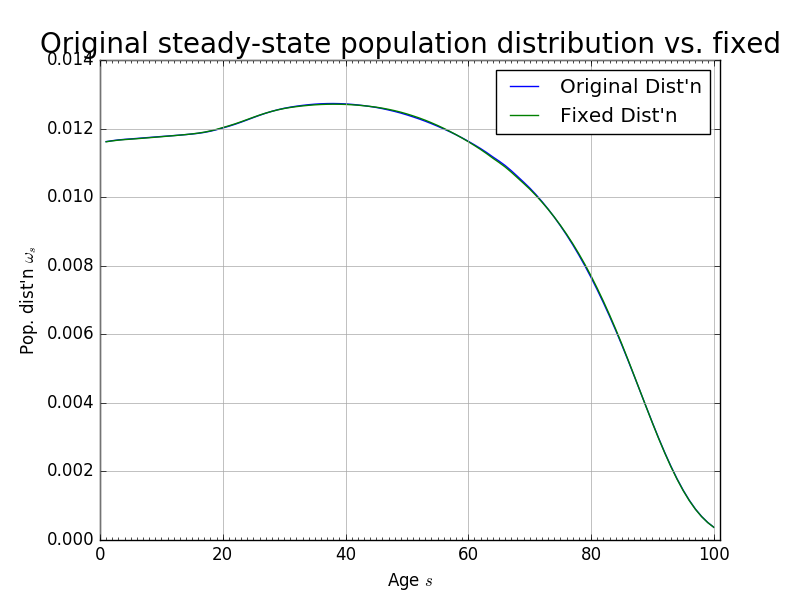
\includegraphics{./images/OrigVsFixSSpop.png}}}
  \end{figure}

  Further, we find that the maximum absolute difference between the population levels $\hat{\omega}_{s,t}$ and $\hat{\omega}_{s,t+1}$ was $1.3852\times 10^{-5}$ after 160 periods. That is to say, that after 160 periods, given the estimated mortality, fertility, and immigration rates, the population has not achieved its steady state. For convergence in our solution method over a reasonable time horizon, we want the population to reach a stationary distribution after $T$ periods. To do this, we artificially impose that the population distribution in period $t=120$ is the steady-state. As can be seen from Figure \ref{FigOrigVsFixSSpop}, this assumption is not very restrictive. Figure \ref{FigImmRateChg} shows the change in immigration rates that would make the period $t=120$ population distribution equal be the steady-state. The maximum absolute difference between any two corresponding immigration rates in Figure \ref{FigImmRateChg} is 0.0028.

  \begin{figure}[htbp]\centering \captionsetup{width=4.0in}
    \caption{\label{FigImmRateChg}\textbf{Original immigration rates vs. adjusted immigration rates to make fixed steady-state population distribution}}
    \fbox{\resizebox{4.0in}{3.0in}{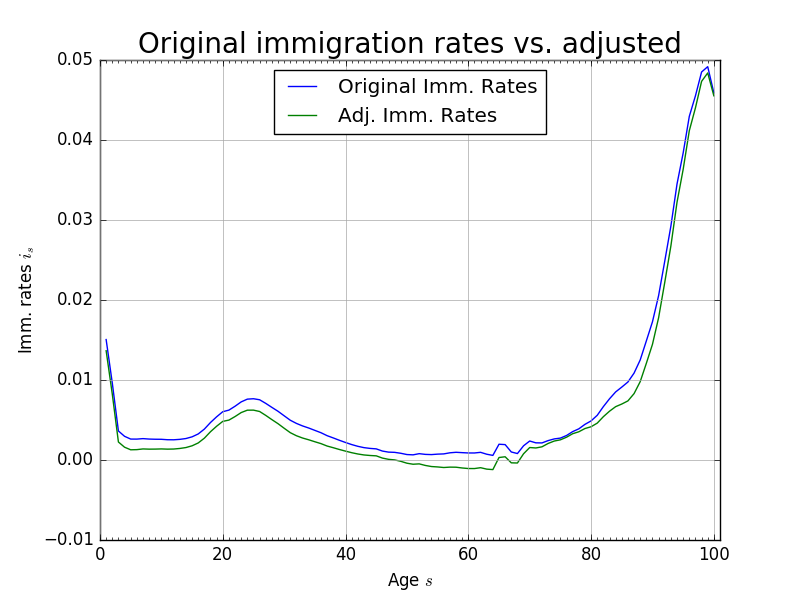
\includegraphics{./images/OrigVsAdjImm.png}}}
  \end{figure}

  The most recent year of population data come from \citet{Census:2015} population estimates for both sexes for 2013. We those data and use the population transition matrix \eqref{EqPopLOMstatmat2} to age it to the current model year of 2015. We then use \eqref{EqPopLOMstatmat2} to generate the transition path of the population distribution over the time period of the model. Figure \ref{FigPopDistPath} shows the progression from the 2013 population data to the fixed steady-state at period $t=120$. The time path of the growth rate of the economically active population $\tilde{g}_{n,t}$ is shown in Figure \ref{FigGrowthPath}.

  \begin{figure}[htbp]\centering \captionsetup{width=4.0in}
    \caption{\label{FigPopDistPath}\textbf{Stationary population distribution at periods along transition path}}
    \fbox{\resizebox{4.0in}{3.0in}{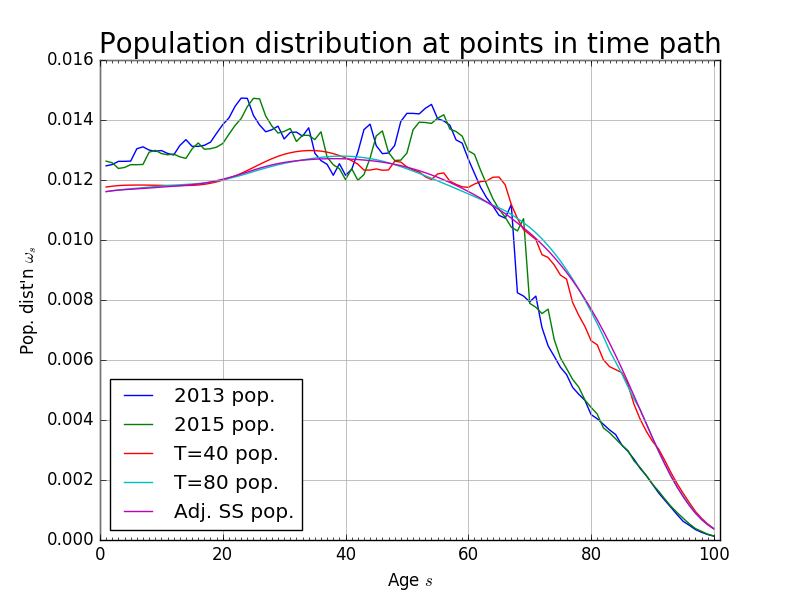
\includegraphics{./images/PopDistPath.png}}}
  \end{figure}

  \begin{figure}[htbp]\centering \captionsetup{width=4.0in}
    \caption{\label{FigGrowthPath}\textbf{Time path of the population growth rate $\tilde{g}_{n,t}$}}
    \fbox{\resizebox{4.0in}{3.0in}{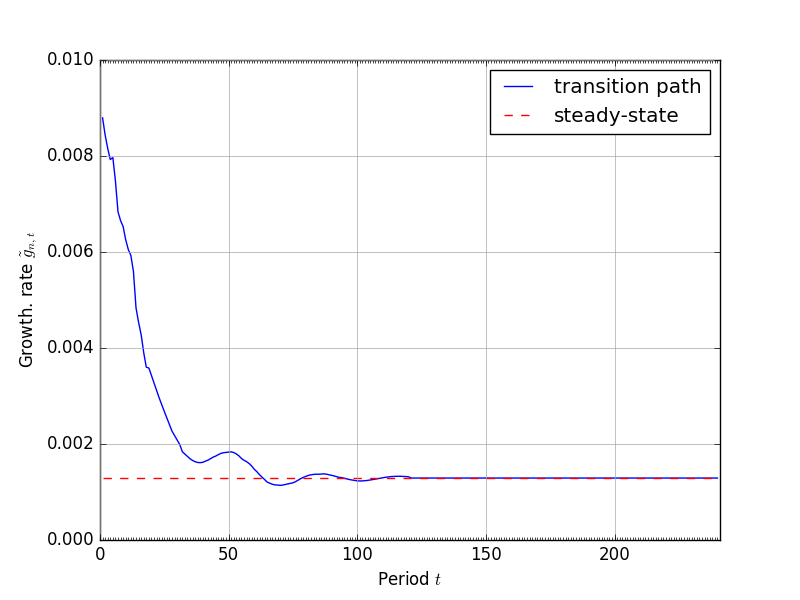
\includegraphics{./images/GrowthPath.png}}}
  \end{figure}
